\subsubsection{\stid{3.06} PETSc-TAO} \label{subsubsect:petsc}
\paragraph{Overview} 

Algebraic solvers (generally nonlinear solvers that use sparse linear solvers) and integrators form the 
core computation of many numerical simulations. No scalable ``black box'' sparse solvers or integrators 
work for all applications, nor are there single implementations that work well for all problem sizes. 
Hence, algebraic solver and integrator packages provide a wide variety of algorithms and implementations 
that can be customized for the application and range of problem sizes. PETSc/TAO~\cite{petsc:homepage,petsc-man} 
is a widely used numerical library for the scalable solution of linear, nonlinear, and variational systems,
for integration of ODE/DAE systems and computation of their adjoints, and for numerical optimization. 
This project focuses on three topics: (1) partially matrix-free scalable solvers to efficiently use 
many-core and GPU-based systems; (2) reduced synchronization algorithms that can scale to larger 
concurrency than solvers with synchronization points; and (3) performance and data structure 
optimizations for all the core data structures to better utilize many-core and GPU-based 
systems as well as provide scalability to the exascale systems.

The availability of systems with over 100 times the processing power of today's machines compels the utilization 
of these systems not just for a single ``forward solve'' (as discussed above), but rather within a tight loop 
of optimization, sensitivity analysis (SA), and uncertain quantification (UQ). This requires the implementation 
of a new scalable library for managing a dynamic hierarchical collection of running scalable simulations, where 
the simulations directly feed results into the optimization, SA, and UQ solvers.  This library, which we call 
libEnsemble, directs the multiple concurrent ``function evaluations'' through the tight coupling and 
feedback. This work consist of two parts: (1) the development of libEnsemble; and (2) the development 
of application-relevant algorithms to utilize libEnsemble.

\paragraph{Key Challenges}

A key challenge for scaling the PETSc/TAO numerical libraries to Exascale systems is that traditional 
``sparse-matrix-based'' techniques for linear, nonlinear, and ODE solvers, as well as optimization 
algorithms, are memory-bandwidth limited.  Another difficulty is that any synchronizations 
required across all compute units---for example, an inner product or a norm---can 
dramatically affect the scaling of the solvers.  Another challenge is the need to
support the variety of accelerators that will be available on the exascale systems
and the programming models that application teams use for performance
portability.

Running an ensemble of simulations requires a coordination layer that handles load balancing and
allows the collection of running simulations to grow and shrink based on feedback. Thus, our
libEnsemble library must be able to dynamically start simulations with different parameters, 
resume simulations to obtain more accurate results, prune running simulations that the solvers 
determine can no longer provide useful information, monitor the progress of the simulations, 
and stop failed or hung simulations, and collect data from the individual simulations both 
while they are running and at the end.

\paragraph{Solution Strategy}

To address the scalability of the numerical libraries, we implemented new solvers and data 
structures including: pipeline Krylov methods that delay the use of the results of inner 
products and norms, allowing overlapping of the reductions and other computation; partially 
matrix-free solvers using high-order methods that have high floating-point-to-memory-access 
ratios and good potential to use many-core and GPU-based systems; and in-node optimizations 
of sparse matrix-matrix products needed by algebraic multigrid to better utilize many-core 
systems.

Our strategy for coordinating ensemble computations has been to develop libEnsemble
to satisfy our needs.  This library should not be confused with workflow-based 
scripting systems; rather it is a library that, through the tight coupling and 
feedback, directs the multiple concurrent ``function evaluations'' needed by 
optimization, SA, and UQ solvers.

\paragraph{Recent Progress}

In the past year, we have released PETSc/TAO 3.14 (available at \url{http://www.mcs.anl.gov/petsc}),
which features enhanced GPU support.  The library now supports CUDA-11 and HIP, along with CUDA-aware 
MPI, which allows direct communication of data between Summit GPUs, bypassing the previously needed 
step of first copying the data to the CPU memory. This enhancement reduces the latency of the 
communication and improves bandwidth.  An experimental Kokkos backend for some matrix and 
vector operations using KokkosKernels was also provided, as one step in the refactoring 
process to support the variety of accelerators needed for exascale systems and the 
programming models for performance portability wanted by applications.

\begin{figure}
\centering
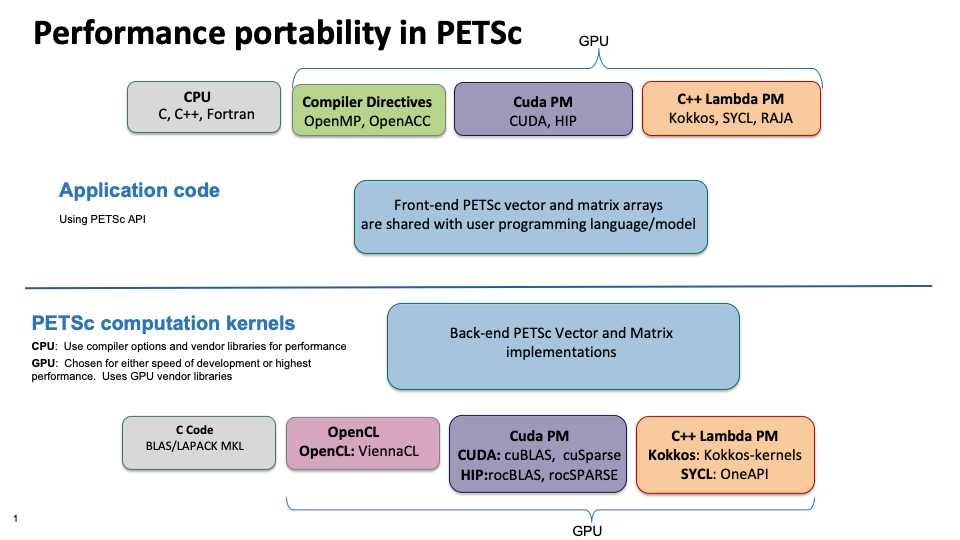
\includegraphics[trim = 0in .2in 1.7in .2in, clip, width=0.9\textwidth]{projects/2.3.3-MathLibs/2.3.3.06-PETSc-TAO/petsc_arch}
\caption{The improved PETSc/TAO architecture enables users to utilize a variety of programming 
models for GPUs independently of PETSc's internal programming model.}
\label{fig:petsc-tao-fig}
\end{figure}

We have also release libEnsemble 0.7.1 (available at \url{https://github.com/Libensemble/libensemble}).
This release includes new generator functions and examples, changes to become xSDK compatible, and 
improved testing across available platforms.

\paragraph{Next Steps}

Our next efforts are:
\begin{enumerate}
  \item \textbf{Performance and application assessment}: 
  We will provide updated performance reports of PETSc/TAO on the architectures available to us.
  We will work with our applications to assess the usage of our software technologies and our 
  progress toward reaching our impact goals.
  We will add a libEnsemble guide for function writer users to the documentation and survey 
  the libEnsemble user community.
  \item \textbf{PETSc/TAO release with full-functionality on available hardware}:
  We will release a version of PETSc/TAO that fully supports the hardware and software on the 
  architectures available to us. 
  We will begin testing important kernels using different backends and prepare more methods to utilize accelerators.
  \item \textbf{libEnsemble release with enhanced capabilities}:
  We will release a version of libEnsemble that implements a method for Bayesian calibration. 
  We will connect libEnsemble to continuous integration tools and demonstrate capabilities.
  \item \textbf{PETSc/TAO release focused on performance on available hardware}:
  We will release a version of PETSc/TAO with performance improvements on the architectures available to us. 
  We will continue testing important kernels using different backends and optimize more methods to 
  utilize accelerators.
\end{enumerate}

